%%%%%%%%%%%%%%%%%%% EJERCICIO 16 %%%%%%

\textbf{Ejemplo 16}\\
Una persona debe pagar  COP  700.000 en 3 meses y  COP  850.000 en 8 meses; ante la imposibilidad de
cancelar las deudas en las fechas previstas le ofrece al acreedor que le cancelara  COP  500.000 en 4
meses y  COP  1'300.000 en 12 meses. Si el acreedor acepta esta nueva forma de pago ¿Qué tasa de
interés periódica mes vencido estará pagando?.\\ \\

%\newpage %USAR SOLO SI EL SOLUCIÓN QUEDA SOLO Y ES NECESARIO BAJARLO A LA SIGUIENTE PAGINA
\textbf{Solución.}\\
%La tabla ira centrada
\begin{center}
  \renewcommand{\arraystretch}{1.5}% Margenes de las celdas
  %Creación de la cuadricula de 3 columnas
  \begin{longtable}[H]{|c|c|c|}
    %Creamos una linea horizontal
    \hline
    %Definimos el color de la primera fila
    \rowcolor[HTML]{FFB183}
    %%%%% INICIO ASIGNACIÓN PERíODO FOCAL %%%%%%%
    %%%%%%%%%% INICIO TITULO
    %Lo que se hace aquí es mezclar las 3 columnas en una sola
    \multicolumn{3}{|c|}{\cellcolor[HTML]{FFB183}\textbf{1. Asignación período focal}}                                                      \\ \hline
    \multicolumn{3}{|c|}{\textbf{ $pf = \textit{ período focal: 0 pmv} $}}                                                                  \\ \hline
    %%%%%%%%%% FIN TITULO
    %%%%% INICIO DECLARACIÓN DE VARIABLES %%%%%%%
    %%%%%%%%%% INICIO TITULO
    %Lo que se hace aquí es mezclar las 3 columnas en una sola
    \multicolumn{3}{|c|}{\cellcolor[HTML]{FFB183}\textbf{2. Declaración de variables}}                                                      \\ \hline
    %%%%%%%%%% FIN TITULO
    %%%%%%%%%% INICIO DE MATEMÁTICAS
    %Cada & hace referencia al paso de la siguiente columna
    $F_{1} =  COP  850.000  $ & $F_{3} =  COP  500.000 $    & $n_ {2} = 8 \textit{ pmv}  $                                                  \\
    $F_{2} =  COP  700.000  $ & $F_{4} =  COP  1'300.000  $ & $n_ {3} = 4 \textit{ pmv}   $                                                 \\
    $i = ?\%  $               & $n_{1} = 3 \textit{ pmv}  $ & $n_ {4} = 12 \textit{ pmv}  $                                                 \\ \hline

    %%%%%%%%%% FIN DE MATEMÁTICAS
    %%%%% FIN DECLARACIÓN DE VARIABLES


    %%%%% INICIO FLUJO DE CAJA
    \rowcolor[HTML]{FFB183}
    \multicolumn{3}{|c|}{\cellcolor[HTML]{FFB183}\textbf{3. Diagrama de flujo de caja}}                                                     \\ \hline
    %Mezclamos 3 columnas y pondremos el dibujo
    %%%%%%%%%%%%% INSERCIÓN DE LA IMAGEN
    %Deberán descargar las imágenes respectivas del drive y pegarlas en la carpeta
    %n_capitulo/img/ejemplos/1/capitulo1ejemplo1.pdf  (el /1/ es el numero del ejemplo)
    \multicolumn{3}{|c|}{ 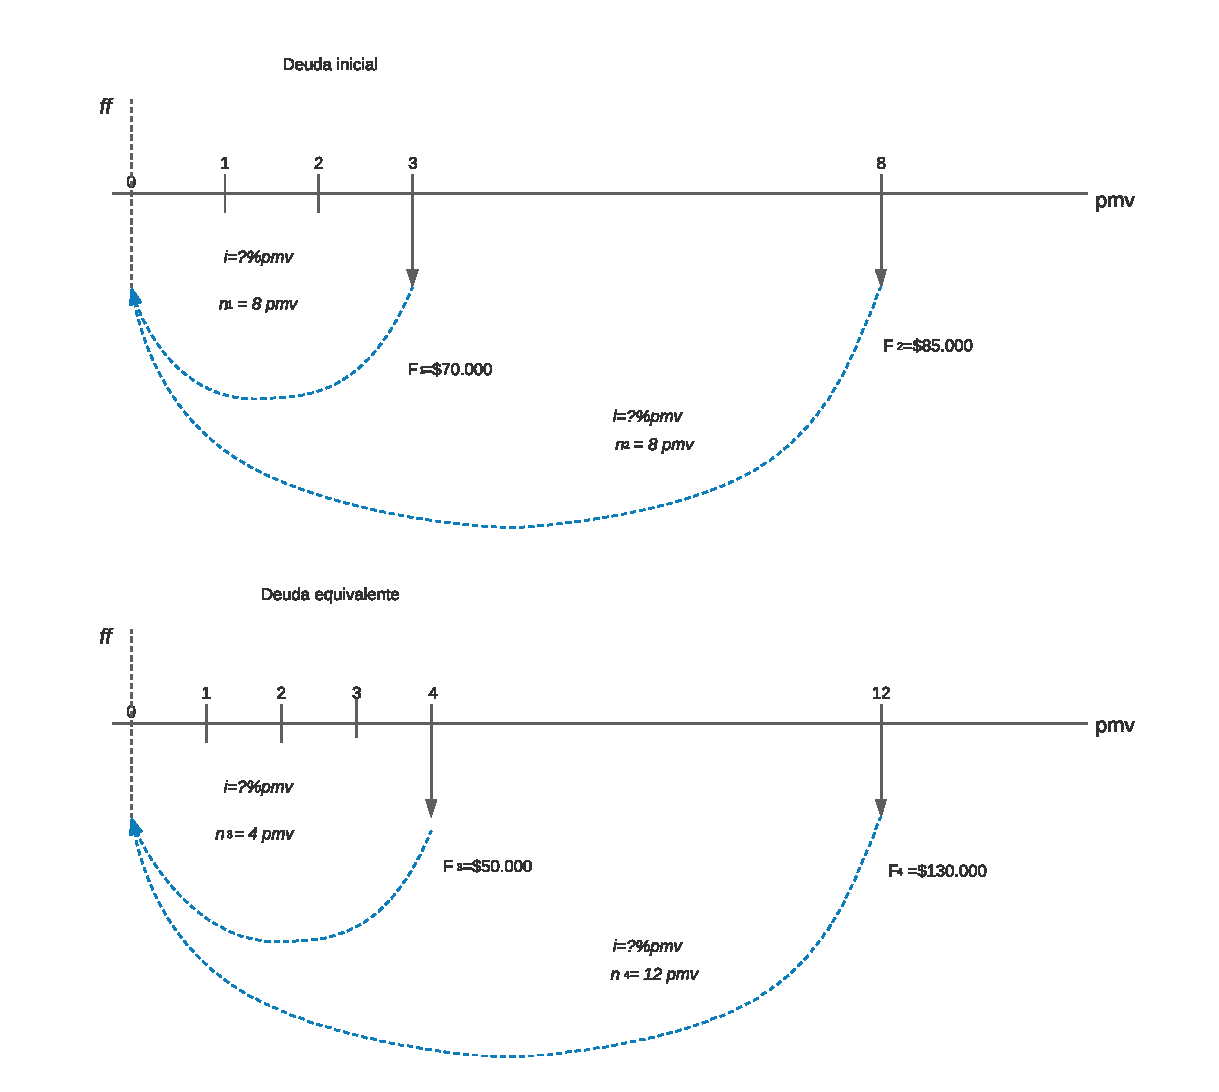
\includegraphics[trim=-5 -5 -5 -5 , scale=0.64]{14/Capitulo2Ejercicio16.pdf} }                                    \\ \\ \hline
    %%%%%%%%%%%%% FIN INSERCIÓN DE IMAGEN
    %%%%%FIN FLUJO DE CAJA



    %%%%% INICIO DECLARACIÓN FORMULAS
    %%%%%%%%%%% INICIO TITULO
    \rowcolor[HTML]{FFB183}
    \multicolumn{3}{|c|}{\cellcolor[HTML]{FFB183}\textbf{4. Declaración de fórmulas}}                                                       \\ \hline
    %%%%%%%%%%% FIN TITULO
    %%%%%%%%%%% INICIO MATEMÁTICAS

    \multicolumn{3}{|c|}{$P = F(1+i)^(-n) \hspace{0.3cm} \textit{Valor presente }$}                                                         \\
    \multicolumn{3}{|c|}{$P_{1} + P_{2} = P_{3} + P_{4} \hspace{0.3cm} \textit{Ecuación de eqv.}$ }                                         \\
    \multicolumn{3}{|c|}{$ $ }                                                                                                              \\
    \multicolumn{3}{|c|}{$ $ }                                                                                                              \\ \hline
    %%%%%%%%%% FIN MATEMÁTICAS
    %%%%%% INICIO DESARROLLO MATEMÁTICO
    \rowcolor[HTML]{FFB183}
    %%%%%%%%%%INICIO TITULO
    \multicolumn{3}{|c|}{\cellcolor[HTML]{FFB183}\textbf{5. Desarrollo matemático}}                                                         \\ \hline
    %%%%%%%%%% FIN TITULO
    %%%%%%%%%% INICIO MATEMÁTICAS


    \multicolumn{3}{|c|}{$  COP  700.000(1+i)^{-3}  +  COP  850.000(1+i)^{-8} =  COP  500.000(1+i)^{-4} +  COP  1'300.000(1+i)^{-12}$}      \\
    \multicolumn{3}{|c|}{$ 70(1+i)^{-3} +85(1+i)^{-8} - 50(1+i)^{-4} - 130(1+i)^{-12} = 0   $ }                                             \\
    \multicolumn{3}{|c|}{$ \textit{Primer ensayo:} $ }                                                                                      \\
    \multicolumn{3}{|c|}{$ i_{1} = 2\% \textit{ pmv} $ }                                                                                    \\
    \multicolumn{3}{|c|}{$  COP 700(1+0,02)^{-3} +  COP 850(1+0,02)^{-8} -  COP 500(1+0,02)^{-4} -  COP 1.300(1+0,02)^{-12} = -101,8714 $ } \\
    \multicolumn{3}{|c|}{$ \textit{Segundo ensayo:} $ }                                                                                     \\
    \multicolumn{3}{|c|}{$ i_{2} = 3\% \textit{ pmv} $ }                                                                                    \\
    \multicolumn{3}{|c|}{$  COP 700(1+0,03)^{-3} + COP 850(1+0,03)^{-8} -  COP 500(1+0,03)^{-4} -  COP 1.300(1+0,03)^{-12} = -44,4404 $ }   \\
    \multicolumn{3}{|c|}{$ \textit{Tercer ensayo:} $ }                                                                                      \\
    \multicolumn{3}{|c|}{$ i_{3} = 4\% \textit{ pmv} $ }                                                                                    \\
    \multicolumn{3}{|c|}{$  COP 700(1+0,04)^{-3} + COP 850(1+0,04)^{-8} - COP 500(1+0,04)^{-4} -  COP 1.300(1+0,04)^{-12} = -4,0058 $ }     \\
    \multicolumn{3}{|c|}{$ 	\textit{ Se toman los resultados correspondientes al 3\% y a 4\% por ser los más cercanos y} $ }                 \\
    \multicolumn{3}{|c|}{$ 	\textit{los que presentan diferente signo y los colocaremos de la siguiente forma:} $ }                          \\
    %\multicolumn{3}{|c|}{ 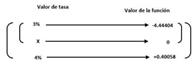
\includegraphics[trim=-5 -5 -5 -5 , scale=0.34]{14/ParteEjercicio16} } \\
    \multicolumn{3}{|c|}{$ \textit{ Se plantea una proporción, teniendo en cuenta las diferencias mostradas en los} $ }                     \\
    \multicolumn{3}{|c|}{$ \textit{corchetes y siempre manteniendo el mismo orden.} $ }                                                     \\
    \multicolumn{3}{|c|}{$ (3-i)/(3-4) = (-4,44404-0)/(-4,44404-0,40058) $ }                                                                \\ \hline


    %%%%%%%%%% FIN MATEMÁTICAS
    %%%%%% FIN DESARROLLO MATEMÁTICO
    %%%%%% INICIO RESPUESTA
    \rowcolor[HTML]{FFB183}
    %%%%%%%%%%INICIO TITULO
    \multicolumn{3}{|c|}{\cellcolor[HTML]{FFB183}\textbf{6. Respuesta}}                                                                     \\ \hline
    %%%%%%%%%% FIN TITULO
    %%%%%%%%%% INICIO RESPUESTA MATEMÁTICA
    \multicolumn{3}{|c|}{

      \begin{minipage}[t][0.07\textheight][c]{0.8\columnwidth}
        $i = 3,91735 \textit{ pmv}$ .
      \end{minipage}
    }                                                                                                                                       \\ \hline


    %%%%%%%%%% FIN MATEMÁTICAS
    %%%%%% FIN RESPUESTA
  \end{longtable}
  %Se crean dos lineas en blanco para que no quede el siguiente texto tan pegado
  %\newline \newline %USARLO SI CREES QUE ES NECESARIO
\end{center}
%%%%%%%%%%%%%%%%%%%%%%%%%%FIN EJERCICIO 16 %%%%%%%%%%%%%%%%%%%%%%%%%%%